\chapter{Hardware and communications}
\label{ch:hardware}
	\section{Introduction}	
	\label{sec:hw-intro}

	%%%%%%%%%%%%%%%%%%%%%%%%%%%%%%%%%%%%%%%%%%%%%%%%%%%%%%%%%%%%%%%%%%%%%%%%%%%%%%%
	% ¡FALTA COMENTAR EN ALGUN SITIO QUE EL DESARROLLO SW SE REALIZA EN PARALELO! %
	%%%%%%%%%%%%%%%%%%%%%%%%%%%%%%%%%%%%%%%%%%%%%%%%%%%%%%%%%%%%%%%%%%%%%%%%%%%%%%%

	%que necesidad cubre la parte hardware del proyecto

	% OLD: The hardware in our project cover a main need, an external device to be able to communicate our android device with a *shimmer through 802.15.4. Than device have to be a little and low powered device that can be conected as device through USB in an android device. Little, because a device that disturb a regular work is not valid at all. Low powered, because if the cost of power the divece is higher than use the stack bluetooth we lose an important advantage of use 802.15.4. Able to be coneced throught USB in our android device because this is the only way to interact with android for a external device. And finally able to be connected as device to elimminate the needed of an extra batery that would have incresed the cost and size of our device. \\

	The hardware research and development part of the project objective is covering a main need: production of an external device that enables communication between an Android system and a Shimmer through 802.15.4. Such a device should be a portable and low-powered device that can be plugged via the widely used USB On-The-Go (USB OTG) to a host Android system, acting the device as a slave.\\

	It has to be small sized because of the target application environment: a particular who requires constant, in-home, ambulatory monitorization. 
	%In that scenario devices that disturb regular working conditions are not valid at all;
	In that scenario unobtrusive operation is a main need, and usual life style activity modification is to be minimized. And it has to be low-powered, because were the power cost of application higher than that of the Bluetooth technology, a main advantage of 802.15.4 is lost.\\ 

	The ability to communicate through USB is required because, at the time, it is the most low battery consuming method to interact with Android powered platforms for any external device[quote here wlan and bt costs].\\

	And finally it should be able to act as the slave in the USB connection to avoid the need of an extra power source for the device that would increase the cost and size of the product.\\

	% OLD: In order to achieve this ambitious goal, we divide this develop in milestones that will help us to focus our works in more concrete tasks and correctly finish the project. \\

	In order to achieve such goals, and being aware of the substancial amount of research involved in this part of the project, the decision is made to adopt a milestone driven development which simplified scheduling and helped focusing on specific tasks while maintaining a global view of the evolution and the objectives of the project.\\

	\section{Overview}
	\label{sec:hw-oview}
	% Before of introduce more infromation about our project we have a section of technologies that will be very usefull to understand all this chapter and that will be referenced many times in other sections

	Before diving any further into the development a section describing technologies involved in the research process is presented, as such information will be key to the understanding of the rest of the chapter and will be throughoutly referenced during the exposition.\\

	Then a description of the hardware research and development process is given, followed by detailed explanation of each projected milestone, including objectives pursued, lines of research developed, results of each one and conclusions obtained. Estimation based decision making being crucial for the correct outcome of the project, special care will be put to explain the motivations for each decision made. The chapter concludes with an exposition of the results of the research and subsequent development.

	%\section{Researched Technologies}
	\section{Technology Research}
	\label{sec:hw-techs}
	%mini introducción diciendo que para la correcta comprensión de está sección surge la necesidad de explicar en mayor o menor profundidad las siguientes tecnologías usadas en algún punto del desarollo del proyecto.

	% The hardware part of this project containts a lot of terms and technologies which is important to know to a correct understanding of the following section but because of it's size we can't explain it whitout a own section because it would become a very heavy doucment and probably lost the reader attencion and the section purpose.

	This part of the project involves a lot of terms and references a number of technologies and concepts which are important to be acquainted with in order to achieve a full understanding of the current chapter. These explanations will not be presented interlaced with the rest of the sections due to the unmanageable size they would acquire leading to a loss of focus which can only act against full comprehension of the exposed content.

		\subsection{Google ADK \& Arduino}
		\label{ssec:Arduino}
			Android Open Accessory Development Kit, referred as ``Google ADK'' or ``ADK'' for now on,
			is a tool set which allows the development of accessories capable of interacting with 
			Android-running devices. It consists of an Arduino board (particularly MegaADK, which is based
			on the ATmega2560 board) and a series of libraries for interacting with an optional set of
			hardware add-ons (``shields''). There are other compatible kits with different boards, like
			NXP-based mbed \cite{mbed}, yet Arduino MegaADK is the one used here.\\
			
			The Google ADK functioning is actually very simple. Regarding the software, it needs of 
			the developing of both an Android application with accessory communication and the board's
			firmware, which models the behaviour of the accessory. Once the board is flashed with its
			firmware, it has to be connected to a power source (through a dedicated wire or Type-B USB)
			and the Android device. If everything is correct, the latter detects the former and, therefore, 
			the accessory starts its operation.\\
			
			Typically, the capabilities of the Arduino board are broaden with the addition of extra shields,
			so that way it can make use of external sensors and agents. The board has multiple input and
			output pins at the developer's disposal as well, so unforeseen behaviours can be achieved.\\
			
		\subsection{MSP430}
		%Posibilidad de tras la epxlicación inicial meter dos secciones más que expliquen las diferencias entre los dos chips y las dos placas usadas(hablarlo todos)
		\label{ssec:msp430}
			MSP430 refers to an entire family of 16-bit CPU microcontrollers from Texas Instruments \cite{msp430}.
			Its most relevant features are:
			\begin{itemize}
				\item \textbf{Very low power consumption:} its several low-power modes make the MSP430 
					family specially suitable for developing embedded systems. Moreover, its brief wakeup 
					transitions from this operating modes are also noteworthy, since these lapses stay 
					around the microsecond ($\mu$s) range.
				\item \textbf{RISC-based Architecture:} its instruction set is particularly narrow \cite{msp430iss}, 
					and thus simple. Reduced instruction sets ease programming when compared to complex ones,
					yet this advantage is not too decisive because of the reason presented next.
				\item \textbf{Simple programming:} Most family members are programmable trough JTAG, which
					makes the debugging process less difficult along with the possibility of swapping
					assembly for C.
				\item \textbf{Wide support and resources:} Texas Instruments provides code examples, software 
					IDEs and thorough documentation as well as it offers extra developing tools like training 
					boards.
			\end{itemize}
			However, it also suffers from some lacks. For instance, MSP430 devices are not equipped with
			external memory bus, what makes flash memory and RAM extensions impossible. In particular, the
			MSP430F66xx family, which the device used within this project belongs to, is provided with only 
			128-256KB of flash storage and 16KB	of RAM --with an extra of 2KB whenever it is not using USB 
			\cite[p. 2]{msp430f6638ds}--. This amount of RAM may be too limited for certain usages (not for 
			this project's particular requirements, though).\\
			
			Concretely, the microcontrollers and boards used in this project are:
			\begin{itemize}
				\item \textbf{Microcontrollers:} \emph{MSP430F5438A} vs. \emph{MSP430F6638}\\
					Both of them are characterized by their low power consumption as well as their voltage 
					range, from 1.8V to 3.6V. Although they share most of their specs, there are some points
					where they differ:
					\begin{enumerate}
						\item \textbf{System Clock Frequency:} in the case of the MSP430F5438A microcontroller
							it is up to 25MHz, whereas MSP430F6638's clock only reaches 20MHz.
						\item \textbf{Wakeup time lapse:} meanwhile TI claims MSP430F5438A wakes from 
							standby mode in less than 5$\mu$s, MSP430F6638 needs less than 3$\mu$s.
					\end{enumerate}
					However, the most important difference lies in the USB support the second microcontroller
					provides, which is the reason why it was chosen for the accessory development. At any rate, 
					full technical specification can be found at \cite{5438a} and \cite{msp430f6638ds} for 
					MSP430F5438A and MSP430F6638, respectively.
				\item \textbf{Boards:} \emph{MSP-EXP430F5438} vs. \emph{MSP-TS430PZ100USB}\\
					MSP-EXP430F5438 \cite{5438aboard} is a prototyping board designed to make use of 
					microcontrollers from the family of MSP430F5438 and stands out for featuring the following 
					sensors and input/output elements: USB, JTAG, 5-position joystick, 2 push-buttons, 
					dot-matrix LCD display, accelerometer... (full list of features in \cite{5438aboard}). 
					Furthermore, it also equips the \emph{CC2420}, 2.4 GHz 802.15.4 radio module, 
					which make this board specially convenient for this project's requirements. This module is
					directly connected to the microcontroller allowing their communication through SPI. In
					addition, its USB connectivity provides a very useful serial output for debugging.\\
					
					% Nonetheless, despite the wide possibilities the previous board offers, the chosen one is
					% the MSP-TS430PZ100USB \cite{6638board}, which is quite simpler, due to its support for the
					% USB-capable MSP430F6638 microcontroller.
					Nonetheless, despite the wide possibilities the previous board offers, the MSP-TS430PZ100USB
					\cite{6638board} is selected. This board lacks serial port output and CC2420 compatible
					sockets, so the connection is to be done by hand and nor any of the other aforementioned
					artifacts available in the MSP-EXP430F5438 is present. But it provides the key feature
					required by the project: the ability to communicate the microprocessor with the board's USB
					connector.
			\end{itemize}
			
		\subsection{Shimmer\texttrademark}
			Shimmer \cite{Shimmer} is a trade name which refers to a wireless sensor platform designed to
			obtain, deal and wirelessly transmit human biological metrics and several ambient and
			kinematic measures. The whole system consists of the Shimmer platform itself and a series of
			extensible sensor modules as its hardware part, an open source firmware library and software
			development tools.\\

			After its proper firmware programming, the platform is capable of retrieving the aforementioned data
			thanks to its expansion modules \cite{ShimmerExp} so that the user can manage it as considers. Once
			the data is appropriately dealt, the Shimmer is able to wirelessly send it via Bluetooth or 802.15.4
			to other receiver nodes, which may be Shimmers or another compatible device.\\

			In order to carry out its tasks, the baseboard of the Shimmer is powered with a MSP430F1611
			microprocessor as CPU, which belongs to the MSP430 microcontroller family previously detailed.
			Additionally, the Shimmer is also equipped with Bluetooth and 802.15.4 radio modules which perform
			the data sending as well as several input/output devices and sensors --three LEDs, one push button,
			accelerometer and a microSD socket, among others--.\\

			Its usage is typically focused on healthcare or remote patient monitoring applications due to its
			small size and weight and its relatively low power consumption (which strongly depends on the
			employment its resources are given). In fact, the manufacturer itself refers to the Shimmer as 
			``wearable wireless sensor platform''. In addition, its multiple sensors allow many other
			applications like athlete performance monitoring or ambient sensing solutions.\\

			This sort of platform is employed at the ECG monitoring project \cite{ESL} developed by the EPFL and
			UCM which, conveniently adapted, performs as the emitter part of the present project. In particular,
			the system described within this document makes use of the 802.15.4 communication capabilities the
			Shimmer platform provides, which mean a key feature of this project.\\

		\subsection{802.15.4}
		\label{ssec:802.15.4}
			The 802.15.4 standard \cite{802.15.4} was first developed by the Institute of Electrical and
			Electronics Engineers (IEEE) in 2003, and was updated with successive revisions in 2006 and 2011.
			This standard sets the specification for the physical layer and Medium Access Control (MAC) of 
			low-rate wireless personal area networks (LR-WPANs \cite[p. 13]{802.15.4}). This sort of networks,
			in the same way that affects WPANs, involves little or no infraestructure, fact that allows the
			implementation of inexpensive and power-efficient solutions for devices of different kinds, when
			compared to more end-user oriented wireless local area networks (WLANs).\\

			As said, this sort of WPANs are intended to be used when having limited power and relaxed throughput
			requirements (concretely, narrow bandwitdth need, up to 250kbps), as they aim for simple,
			easy-to-install short-range networks with little power consumption and low budget. To meet these
			objectives and requirements, the 802.15.4 standard makes use of one or more of the following
			unlicensed bands:

			\begin{itemize}
				\item 868-868.6MHz in Europe.
				\item 902-928MHz in North America.
				\item 2400-2483.5MHz can be employed worldwide.
			\end{itemize}

			Two kind of devices are considered within the standard: full-function (FFD) and reduced-function
			devices (RFD). FFDs are capable of communicating with both other FFDs and RFDs, whereas RFDs can only
			communicate with FFDs (RFDs are supposed to have very simple responsibilities, minimal resources and,
			consequently, send little amounts of data). These devices are to be arranged in peer-to-peer or star
			topologies. Concretely, devices in this project are arranged using a star topology where Shimmer
			emmiter nodes are RFDs which communicate with the receiver node FFD, the MSP430-based device
			connected to the Android tablet.\\

			Regarding the MAC layer, it allows the usage of superframes instead of discrete frames. A superframe
			is bounded between two beacons sent by the FFD coordinator, which also defines the format of the
			superframe. The lapse between two consecutive beacons is equally divided into 16 slots, and may or may
			not be divide into an active and an inactive period, in which the coordinator may enter a low-power
			mode. Particularly, in this project, part of the superframe is divide into portions called guaranteed
			time slots (GTSs), which form the contention-free period (CFP) at the end of the superframe, after
			the contention access period (CAP), as it is represented in \autoref{fig:superframe}. One GTS can use
			more than one slot, but the emitter device has to ensure that its transfer is completed before the
			end of its GTS or the CFP.

			\begin{figure}[h]
				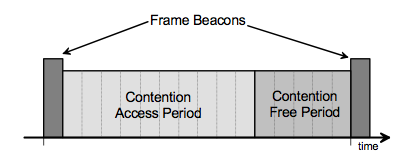
\includegraphics[scale=.5]{superframe}
				\centering
				\caption{Superframe structure with GTSs}
				\label{fig:superframe}
			\end{figure}

			Further information and thorough details about the MAC layer and its frames and superframes
			possibilities and formats can be found at \cite[p. 67]{802.15.4}.\\

			Depending on the direction of the data flow and the usage of beacons or their absence, there
			are three modes of data transferring \cite[p. 18]{802.15.4}, with additional variants according to
			the possible requirement of transfer acknowledgement. In the case of this project, whenever a emitter
			device has data to transfer, it listens the network waiting for a beacon and, once found, it
			synchronizes with the superframe, sending its information in its corresponding GTS. This process is
			illustrated in \autoref{fig:trans-process} (notice that, in this particular case, acknowledgment is
			not required). \todo{Check this.}

			\begin{figure}[h]
				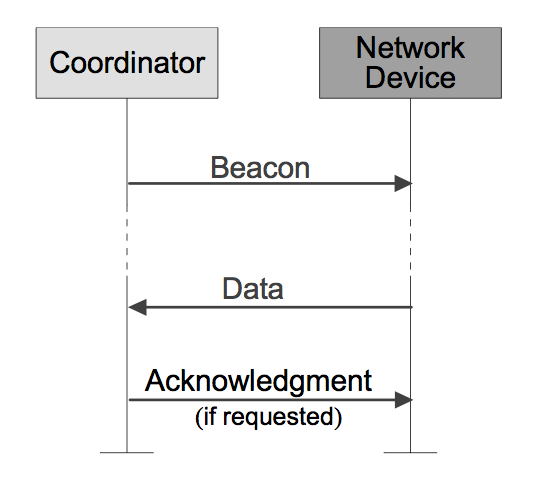
\includegraphics[scale=.4]{trans-process}
				\centering
				\caption{Communication to a coordinator in a beacon-enabled PAN}
				\label{fig:trans-process}
			\end{figure}

			Due to the possibility of *[shutting down/entering low-power mode] this standard provides during the
			lapse of CAP, it allows significant power saving. In \autoref{fig:bcn-recp} and 
			\autoref{fig:bcn-gts-recp} it can be seen that the Shimmer's power consumption significantly drops
			after the reception of the beacon. Two and three clearly different phases, respectively, can be
			observed in both figures:

			\todo{Argue this.}
			\begin{enumerate}
				\item \textbf{Beacon Reception:} first part, which lasts 1.39ms and averages 72.39mW, corresponds
					to the radio entering reception mode when the beacon is expected. Second part consists of
					the beacon reception itself, and it lasts 0.97ms and averages 82.59mW.
				\item \textbf{Low-power mode:} the radio keeps its power consumption to a minimum until its GTS,
					if any packet is to be sent, or till the following beacon.
				\item \textbf{Packet transmission:} (only in \autoref{fig:bcn-gts-recp}) first part is due to the
					sending of the package from the microcontroller to the radio chip, which is still idle 
					(16.8mW, 2.85ms). Second part corresponds to the actual transmission of the packet, which
					averages 51.92mW for 4.51ms.
			\end{enumerate}

			These results were obtained by measuring the voltage at a resistor which was specifically placed
			in the emitter node's power path, as it is detailed in \cite{ecg.del.paper}.

			%(from 0 to 5ms), almost reaching zero mW as base value (peaks are
			%due to ...\todo{Informarse de esto}); keeps at its lowest value till its GTS activates (from 16 to
			%24ms), when it raises again to \todo{Add specific values} during the transmission.

			\begin{figure}[h]
				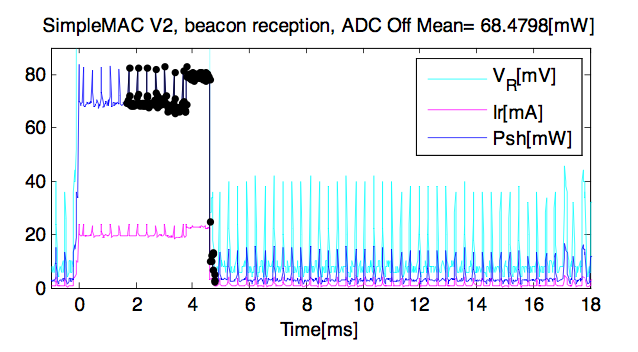
\includegraphics[scale=.4]{bcn-recp}
				\centering
				\caption{Shimmer power consumption analysis, beacon reception}
				\label{fig:bcn-recp}
			\end{figure}

			\begin{figure}[h]
				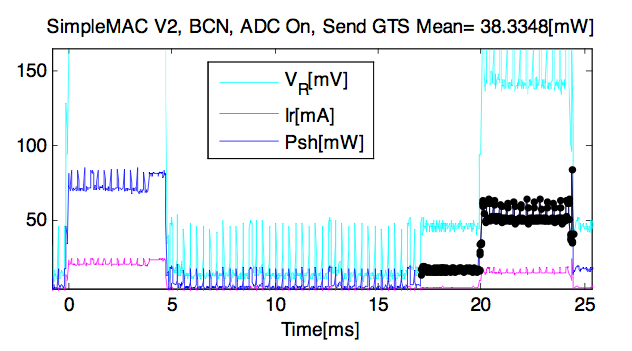
\includegraphics[scale=.4]{bcn-gts-recp}
				\centering
				\caption{Shimmer power consumption analysis, beacon reception and data transmission}
				\label{fig:bcn-gts-recp}
			\end{figure}

			\todo{Compare with Bluetooth power values?}
			These low-power periods grant a much better battery life when compared to the one Bluetooh, as the
			wireless alternative Shimmer provides, allows because of the constant user and protocol data flow
			that it causes, fact that is aggravated by its much broader bandwitdth. Thus, it provokes that the
			average Shimmer battery life employing 802.15.4 is up to two orders of magnitude higher than employing
			Bluetooth. \todo{Assure this.} For instance, a fully loaded battery would increase its life from
			several hours to several days, which would be particularly interesting as it would let its
			replacement not to be a constant nuisance. \todo{Substitute with accurate values.}


		\subsection{FreeRTOS}
		\label{ssec:FreeRTOS}
		\todo{hardware subsection: FreeRTOS technology}
		\todo{Pedir información y referencias a joaquin}
		\subsection{USB device \& USB host}
			USB host \cite{usbhost}, as oppose to USB accessory, is an operation mode which determines how a
			USB-equipped device interacts with another one. The two connected devices are differently named
			according to the role they assume in a host or accessory mode connection, namely USB host and USB
			device. This designation is based on the role each device is playing rather than the sort it belongs
			to. In particular, one end is named USB host if its apparatus is responsible of supplying power to
			the one at the other end.\\

			The main difference between both modes lies within the direction the power supply follows or, more
			specifically, the role the Android running device adopts: Android device acts as host in USB host
			mode, whereas it acts as device in accessory mode. However, there is no difference in data transfer
			between them, as it remains bidirectional in both modes. It is typical that the device with larger
			power consumption (usually the Android device) is the USB host since it probably has a power source
			of any kind, although this is no always this way.\\

			In addition, when in USB host mode, creating the connection, that is, instatiating and initializing
			the proper sockets, between both ends is responsibility of the host, along with notifying the other
			end about the establishment of the communication. On the other hand, the process the end acting as
			device has to carry out is quite simpler, as it just consists of checking the availability of the
			previously created communication.\\

			Regarding this project, this matter applies in the way both the Android and the receiver devices are
			connected and which one assumes the USB host role. It would result particularly desirable that the
			Android device acted as host so that the receiver could be fed from its battery --which would make the
			collection really portable, non-dependent on the accessory power source--. However, it depends on
			the platform that this arrangement can be possible.\\

			Although certain Android devices running version 2.3 were capable of offering USB host support, this
			version only officially supports USB accessory mode; whereas USB host mode is only available by
			default since version 3.1. Thus, in order to get the required behaviour the usage of one of this
			special devices or, preferably, a device running a 3.1 Android version or newer.

	\section{Description}
	\label{sec:hw-descr}

	%Esta parte es el cuerpo de la parte de investigación del proyecto, no se sabía si se podía, no se sabía cómo hacerlo, …

	% The hardware is the center section of the research in the whole project, not because there wasn't more research, but because nobody has researched this areas. At the begining we just know what we want to do but we have absolutely nor idea or clues about how we can do a very important number of our *milestones. In any cases we don't even know if our goals could be achieved, in particular a very important one, we need to connect a MSP430 to a Android where Android acts as host, and nobody achieve this before and therefore there are no information about that in forums or TI official support.\\

	The hardware related investigation is the main section of the research part of the project. Not that there wasn't any research involved in other areas, but some critical elements of this part had never been researched before. 
	At the beginning of the project specific objectives were established and main milestones elected, but absolutely no clue or direction for most of those milestones was available.
	Moreover, in some cases the feasibility of the proposed goals was unknown. Specifically the achievement of the very important objective of USB communication between an [TI's] MSP430 %(ponemos algo más de info o ya se sabe el modelo y todo?) 
	and an Android powered device assuming the latter the role of master and acting the former as a slave was something not done before and therefore no information was available  even in the Texas Instrument support site.\\

	%Plantea un reto porque toca todos los niveles, desde diseño de PCB a nivel componente hasta desarrollo a nivel de SO (kernel? <= investigar si kernel o SO)

	% The project suppose a chalenge because it involves every hardware level, form the lower levels as the PCB design of a device to higher levels as develop parts of a SO. *Aqui molaria poner algo más que dos tristes lineas. \\

	This whole development and research poses some quite interesting challenges as it involves working nearly at every abstraction layer present on device development, ranging from schematic capture and PCB design to operating system related development. The main issues to be resolved are:
	% La idea es refactorizar un poco lo que había en la scrap zone, introducir los puntos que debe resolver
	% el accesorio y después dar paso a los hitos, donde se relaciona cada uno con estos objetivos.
	\begin{itemize}
		\item \textbf{802.15.4 radio reception:}
			data packets are emitted from the monitoring Shimmer\texttrademark and are to be received and dealt
			by the accessory. In order to do so, FreeRTOS has to be equipped with a working implementation of
			the radio stack, which involves implementing part of ZigBee's MAC layer, described by IEEE 802.15.4, 
			as it is the underlying standard which the emitter nodes are based on. 
		\item \textbf{MSP430 USB handling:}
			just as the radio stack, FreeRTOS is not prepared to make use of the USB interface with which the MSP430
			board --namely TS430PZ100USB-- is equipped. Thus, it is necessary to add the essential code in order to 
			incorporate this functionality to the OS. This issue, in the same way as the previous one, is a critical 
			part for the system to work properly since it may likely be a source of errors unless it is perfectly 
			made --for instance, it could add transmission lags, packet corruption or loss--. 
		\item \textbf{MSP430-Android communication:}
			this issue is particularly relevant as no project has ever claimed to feature this kind of
			connection before. Hence, it means an additional challenge to be overcome since it will involve
			the modification or complete development of an specific driver for the MSP430-equipped device.
			This challenge is imposed by choosing the USB host alternative so that the Android device powers
			the accessory. On the other hand, USB device may ease this issue due to the already resolved 
			communication system with accessories made by Google, yet it implies the accessory will need
			an additional power source.
			Fortunately, it finally turned out not to be so tough as it was expected and the goals related
			to this issue were successfully fulfilled, as it can be read at \autoref{ssec:Android.USB}, 
			\nameref{ssec:Android.USB}.
	\end{itemize}
	
	% Let us present the following section...
	Over the following lines within the next section, the aforementioned challenges are detailed
	in the context of their own development stages. In addition, objectives and results of each one of
	these stages are also presented.
	
	\section{Milestones}
	\label{sec:hw-mstones}
	Due to the fair amount of time a essentially researching work like this hardware development will
	require, the foreseen schedule is subject to changes which may completely alter it regardless of 
	how irrelevant they may seem, and thus avoid the success of the project.\\
	
	Keeping this risk in mind, the hardware development was planned as a sequence of milestones,
	ordered by increasing complexity. Every milestone introduces a new technology, each one of them
	capable of covering the needs of the project in a more complete way. In other words, the previously
	presented issues are to be resolved as these stages are overcome.\\
	
	The schedule, then, starts with the usage of the Google Open Accessory Development Kit, based on Arduino,
	in order to make a prototype as first approach and, in this way, be able to parallelize software and
	hardware development --notice that both of them depend on each other--. This choice is made because of
	the well-known soft learning curve Arduino presents as well as the already prepared connection
	the Google ADK provides between accessories and Android devices.\\
	
	The next step in the development, once the application has been proven to communicate with a data-providing
	accessory, consists of making Android capable of detecting and communicate via USB with an MSP430-equipped
	device. This stage can be qualified as very critical, since almost every part of the development
	depends on it.\\
	
	The following milestone arises as a consequence of the FreeRTOS port which was specified before: its
	target device, namely MSP430F5438A, does not support USB communication, and by extension the port itself.
	Thus, the work for this stage consists of providing FreeRTOS with USB support, which is to be employed
	with the new target device, MSP430F6638, which is member of the MSP430F66xx family with highest performance,
	along with USB support.\\
	
	Next, the planning set the development of the communication between the emitter nodes and the device.
	The previously existing FreeRTOS port already supports the IEEE 802.15.4 standard MAC layer, so the
	work in this milestone involves needed modifications in order to get the port work properly with
	the new platform MSP430F6638. Although the first versions of the schedule considered this next step 
	at the same time of the previous one, in later revisions it was decided to keep them separated for 
	the sake of stability, derived from isolating both developments.\\
	
	Due to the division between the two previous stages, both developments, USB and radio stacks, are
	to be done separately. In order to resolve the likely communication problems this decision can cause,
	the next iteration the planning considers is reserved for validating and fixing their coexistence
	may provoke.\\
	
	Finally, the schedule adds two extra stages: the first, which may be dropped due to eventualities,
	considers the design of a miniaturized version of the receiver device so as to dispense with the
	TS430PZ100USB board, which is rather big and little portable. The second one is essential as it
	is reserved for possible needed fixings and refinements.\\
	\todo{¿Tabla con las fechas de inicio y fin de las milestones?}
	
	All these stages are now detailed over the following subsections.\\

	\subsection{Arduino for Android USB Device Comunication}
	\label{ssec:Arduino.USB}
		The objectives for this first milestone objectives are:
		\begin{itemize}
			\item acquire a suitable Android device prototyping environment, 
			\item manage correct communication between Android and a prototype device, and
			\item develop an application emulating desired behaviour.
		\end{itemize}
			
		% Milestone justification
		This milestone is set upon the consideration that it is a good approach in order to familiarize
		the team with communications between Android and USB devices. It also comes motivated by the
		previously supposed effort the connection between Android and an MSP430-equipped device involves,
		since it has not been done before as well as Android USB host mode support has been out for only
		two months.\\

		The process involved in the procurement of each objective is exposed next.

		\begin{enumerate}
			\item \emph{Acquire a suitable Android device prototyping environment}\\
				The first step in order to develop this USB device consists of looking for a platform which
				is able to provide the needed components and libraries so as to make the connection with
				Android feasible. Although several devices are available to serve as Android accessories (as
				it is explained at \autoref{ssec:Arduino}),	Google ADK is the chose one since it is based on
				Arduino: a considerable amount of libraries and documentation is to be expected. Particularly,
				USB host mode library is the main reason for choosing it.

			\item \emph{Manage correct communication between Android and a prototype device}\\
				Once the target platform is chosen, the next step to be done consists of developing some
				test firmware for the Arduino as well as modifying consistently the Android application
				so that a proper communication between both devices can be established and proven. A period 
				of learning and adaptation is required for the team to achieve this.

			\item \emph{Develop an application emulating desired behaviour}\\
				For this milestone to be fulfilled, it is required that the firmware developed for the
				Arduino can emulate the behaviour of an actual sample-receiving device. Thus, the
				microcontroller board is programmed in order that it sends formatted data as the Android
				application is expecting to receive. In this way, it is visually verifiable that the
				data transmission is performing properly.
		\end{enumerate}

		Although Google refers its ADK as an accessory developing platform, it is noticeable that it is
		in fact used as a prototyping tool, and hence this development is not to be employed as a part
		of the final state of the system. As opposed to this, this stage of the project is considered as
		training transition to more technical developments to be engaged later.

	\subsection{MSP430 for Android USB Host Comunication}
	\label{ssec:Android.USB}
		Objectives for this stage are:
		\begin{itemize}
			\item supply MSP430 with USB protocol application functionality,
			\item research Android USB protocol related functionality,
			\item make Android OS recognize MSP430 when plugged, and
			\item manage communication between Android and MSP430 via USB.
		\end{itemize}

		Due to the need of USB support, both the microcontroller and its board models are required to be
		as new as possible, since older models lack this feature. Therefore, the MSP430F6638 microcontroller
		as well as the MSP-TS430PZ100USB board are selected for this development, as it is explained at
		\autoref{ssec:msp430}, \nameref{ssec:msp430}.\\
		
		Prototyping with Arduino during the previous milestone constitutes the preparation for the development
		to be done in the present one. Yet, whereas Android and Google ADK are designed to interact with
		one another, Android is not prepared for supporting a device like an MSP430 out of the box. So, in order
		to communicate both devices, an API from Texas Instruments \cite{TIUSB} is the only available tool, though
		it is designed for Windows OS.\\
		
		Among all the contents the TI API includes, its examples result particularly useful for the project
		requirements. Concretely, examples about CDC (Communications Device Class) protocol set the needed
		basis to fulfill the objectives for this milestone. Nonetheless, several examples does not seem to
		function, not even in Windows, its target operating system. Thus, the next step consists of studying
		both the examples and documentation from TI so as to fulfill the objectives.\\
		
		\begin{enumerate}
			\item \emph{Supply MSP430 with USB protocol application functionality}\\
				As it was previously said, TI API contains a huge amount of information in the shape of:
				\begin{itemize}
					\item \textbf{Extense documentation:} about the API itself and features of TI devices. 
					\item \textbf{Sample Windows Applications:} made to communicate Windows PCs with external
						devices or enumeration tools.
					\item \textbf{Suite of examples:} each of them implements a combination or one of the
						following USB protocols: Communications Device Class (CDC), Human Interface Device (HID)
						or Mass Storage Class (MSC).
				\end{itemize}
				
				The same problems, though, keep these examples from working with the target MSP430 device. As a
				result of an intense investigation the trouble is found to lie within one of the device's clocks
				which, according to the API documentation, may need an specific tuning --particularly, 4MHz--.
				Moreover, in spite of the fact that the board seems functional, it actually lacks that certain
				clock. As expected, TI example properly works with the addition of the 4MHz clock.\\
				
				In addition to the previous hitch, another one arises upon changing the current workstation.
				Every work during this development is carried out within a Windows virtual machine running over
				Windows, yet the examples stops working when the host machine is changed for another one running
				GNU/Linux, particularly Ubuntu. Despite having achieved the present objective, this fact reduces
				the expectations for the next one since Android, the target OS, is also based on Linux kernel.\\
				
			\item \emph{Research Android USB protocol related functionality}\\
				As it is expected because of its performance with Ubuntu, Android is not able to recognize the
				target device, and hence the example cannot be tested. In order to solve this inconvenience, two
				solutions are considered: search for the proper driver, if any, and modify it or develop
				it from scratch.\\
				
				Nevertheless, the search concludes with no results, so it is assumed that this particular driver
				does not exist. The most similar resource found consists of a driver for MAC OS X, which would
				have to be consistently modified in order to make it work. However, this idea is dropped due to
				the advice obtained from a qualified source that suggests exploring other methods to make the
				communication feasible apart from developing a driver, which may be too harsh and spend too much
				time. A quite considerable risk is assumed by doing so as there are no warranties of finding a
				proper solution.\\
				
				Fortunately, further research drives to a successful alternative: it is found that Android
				actually implements HID protocol, which is also supported by MSP430 through the Texas Instruments
				API. Finally, upon loading the proper HID application into the MSP430 from the TI API this
				objective reaches its fulfillment.\\

			\item \emph{Make Android OS recognize MSP430 when plugged}\\
				Once both two first objectives of this milestone are achieved, MSP430 recognition by Android is
				inmediate when the connection is set since all the needed work is already done.\\

			\item \emph{Manage communication between Android and MSP430 via USB}\\
				At this point, the work still to be done consist of modifying the Android application in order
				that it can read data from the receiver device. However, this is not a trivial work as Android
				USB host communication is highly dependant on the device which it has to read from. Thorough
				investigation over the API manuals is required to discover every detail and make it work.\\

		\end{enumerate}

		Therefore, as it can be deduced from the previously explained happenings, this stage draws a great amount 
		of risk to the hardware development due to several critical points it involves which further required
		tasks are to be based on. In other words, part of this project's probabilities of success greatly depends
		on the feasibily of the present objectives, so this milestone completely conditions the planning. Once 
		it is finished, it will certainly allow to tune the schedule with better accuracy.\\

	\subsection{USB in FreeRTOS}
	\label{ssec:USB.FreeRTOS}	
		This milestone's objectives are:
		\begin{itemize}
			\item check the proper working of FreeRTOS with the new microcontroller,
			\item validate the feasibility of the usage of USB API along with FreeRTOS in MSP430,
			\item correctly integrate USB API into FreeRTOS, and
			\item manage USB data sending in FreeRTOS.
		% REALIZACION: port testing application to FreeRTOS task system.
		\end{itemize}

		Despite having already achieved communication between Android and MSP430 device through USB, there is
		still work about this since it is only a test version which does not take FreeRTOS into account. In fact,
		FreeRTOS, as it is explained at \autoref{ssec:FreeRTOS}, will be responsible of managing the operation of
		the microcontroller in addition to the radio. So, adapting the USB functionality and equipping FreeRTOS
		with it arises as the next relevant stage of the project, required to make the receiver device possible.\\

		\begin{enumerate}
			\item \emph{Check the proper working of FreeRTOS with the new microcontroller}\\
				Prior to starting with this milestone's core objective, FreeRTOS needs to be adapted in order to
				make it work with the new microcontroller, namely MSP430F6638, since it is addressed to a
				different model, the MSP430F5438A. This change implies the modification at several points of the
				code of the operating system so that its proper working can be assured.\\

			\item \emph{Validate the feasibility of the usage of USB API along with FreeRTOS in MSP430}\\
				The following objective to be achieved consists on incorporating the TI USB API to FreeRTOS,
				focusing in its completion rather than its perfect working. This is not a trivial task due to the
				large extension of API's code. Furthermore, The most relevant inconvenience that endangers this
				work is the considerable amount of resources which are found to be in mutually exclusive
				condition, such as microcontroller pins and clocks. However, this is a matter of properly
				balancing the distribution of these resources over time, and thus it can be achieved by paying
				special attention and care to it.\\

			\item \emph{Correctly integrate USB API into FreeRTOS}\\
				Although the USB API is already functional and integrated into FreeRTOS, this integration is made
				without caring about keeping the compatibility with already supported microcontrollers, and hence
				losing this feature. Therefore, the next step consists of restoring its support for other devices
				like MSP430F5438A. Nonetheless, as the original FreeRTOS port already supported different devices
				such as the one mentioned and Shimmer\texttrademark, this work is not as hard as it should be if
				carried out analogously.\\

			\item \emph{Manage USB data sending in FreeRTOS}\\
				Once the USB functionality is properly integrated into FreeRTOS, it is required to check whether
				the communication it provides correctly stablishes and the trasmitted data does not suffer from
				corruption or loss. The method used to test this consists of running a special program on FreeRTOS
				which sends a known character sequence so the input and output sequence can be checked as equal.
				As they are, in fact, the same sequence, this objetive along with the entire milestone are
				fulfilled.\\

		\end{enumerate}

		With the work carried out during this stage, communication between the receiver and the Android device is
		completed, fact that limits the work that is left to to the management of the wireless reception through
		802.15.4. Wireless communication will be dealt over the following two milestones.\\

	\subsection{802.15.4 in FreeRTOS}
	\label{ssec:802.15.4.FreeRTOS}	
		This milestone's objectives are:
		\begin{itemize}
		\item validate current implementation of 802.15.4 in FreeRTOS in MSP430 testing board,
		\item manage connection to the CC2420 radio module to target MSP430 device,
		\item port implementation of 802.15.4 to target MSP430 device, and
		\item prepare such implementation for actual usage.
		\end{itemize}

		%Estado de la capa MAC
		% At the beginining of this milestone there are a port of the needed part of the MAC layer of the 802.15.4, that have been tested in just certain conditions, like send of medium lenght packets.\\
		The next step is the achievement of wireless 802.15.4 receiving in the MSP430 board through the CC2420 radio module. An existing port of the MAC layer \todo{developed by jrecas, indicate?} for the FreeRTOS running in the MSP430 is taken as the starting point. The main advantage of employing it is that it's the same code running in the 802.15.4 emitter utilized in the project. In any case, before actual usage a correct validation of the software is mandatory. Once validation is completed, the MAC layer is to be implemented into the target MSP430 device and tweaked for actual usage. That is the ultimate goal of this milestone.\\

		\begin{enumerate}
		\item \emph{Validate current implementation of 802.15.4 in FreeRTOS in MSP430 testing board}\\
		%Radio probada en una placa que no proveía USB pero sí salida por puerto serie para simplificar trabajo y facilitar la depuración,		

		% As we are not sure of the right working of MAC layer in our system we decide to test it with the old board and microchip that provides serial port output that is extreamly usefull in the debug of a real-time system like this. This result to not works for a certain problems as although it's able to recibe 802.15.4 packets it's not programmed to it, and the max size packets wasn't recived correctly.\\

		Before addressing the delicate task of implementing the 802.15.4 MAC layer port into the target MSP430 device, validation of this port is conducted in the testing MSP430F5438A board. This decision is motivated by the fact that this board provides serial port output and out of the box CC2420 connection.\\

		The testing of the MAC layer provides negative results, as although 802.15.4 receiving functionality is present in the port, the OS is not actually notified about it and the received data is lost. Moreover, problems in the receiving of packages of maximum size, which are the ones sent by the 802.15.4 emissor, are also detected.\\

		The amendment of the aforementioned problems takes no longer that expected, and the porting of the 802.14.4 support to the target MSP430 device begins. The original developer of both the FreeRTOS port and the MAC layer is notified about the detected problems, and the fixes are also implemented on the 802.15.4 emissor.\todo{this would be jrecas}\\

		%se llevó luego a otra con USB pero sin soporte ni software ni hardware para la radio, obligando a mapeo manual de pines,
		\item\emph{Manage connection to the CC2420 radio module to target MSP430 device}\\

		% Once the right working of the MAC layer is tested, it's time to port it to the new board and microchip, that implies a lot of troubles because the TS430PZ100USB have no conection to a CC2420 radio module. This mean that a full study of the 100 aviable pins to discover which ones are actually unused by both the SO and USB comunication. The radio modlule alse need a particular kind of pins in some cases that there are no very abundant. With this study and the mapping of pins made\todo{(mencionamos a carlos aqui?)} board and radio module is sent to be weld.\\

		The target MSP430PZ100USB board provides no CC2420 radio module connection socket, so the port of the validated 802.15.4 module to this board requires manual connection handling of the radio device. The MSP430 features a 100-pin footprint, and a complete study of all the 100 pins target usage and on-board availability becomes mandatory for the identification of the pins that the CC2420 will be connected to. Special care is put to avoid collisions between the USB and the radio modules regarding hardware resources.\\

		Successful identification of the required pins done, a manual soldering of the CC2420 radio module is executed \todo{by dixon} and subsequent testing can continue.\\

		\item\emph{Port implementation of 802.15.4 to target MSP430 device}\\

		%que ahora si con más mañana que suerte se hizo bien y no dio conflicto como veremos ahora aunque si hubo que modificar algo más de código dado que la nueva placa necesitaba iniciar los pines de la radio de otra forma.
		% While the board is available, we addressed the programming the pin mapping for de MSP430F6638 into it's class in the FreeRTOS using as base the MSP430F5438A pin mapping class. This is a particulary delicated code and was carefully developed, because if just one thing is not perfect the radio simply didn't work at all and the potencial error will be hard to discover. \\
		The inclusion of the 802.15.4 MAC layer into the target MSP430 device involves modifing the FreeRTOS pin mapping code, which is a specially sensitive task. The code is carefully modified taking the mapping code for the already tested MSP430F5438A as the base. Special care is put in the task as any mistake would cause the radio module to fail at initialization and following error tracking would be very time consuming. \\

		Once the FreeRTOS pin mapping is complete, no further work is, initally, required in the port process.\\

		\item\emph{Prepare 802.15.4 implementation for actual usage}\\

		% No va, había que cambiar un par de cosas en la inicialización, lo descubrimos en un ejemplo de TI
		% With both, board and codding finished the radio was tested and it didn't even trun on. The answer to this trouble was found in a code examples provided by TI for the MSP430F6638, specifically in the \textit{Universal Asyncronous Reciver/Transmiter(USART) initialization code} that reslut to differ slightly of the old MSP430 USART initialization.\\

		Having both the hardware and the software part of the 802.15.4 module port completed, actual testing is conducted on the target MSP430 device, resulting in an initial absolute failure. The radio module nor even turning on, an in-depth research on the subject becomes the main priority.\\

		The solution is found in one of the TI code examples for the target MSP430, which provides a different code for the Universal Receiver/Transmitter (USART) initialization routine than the one employed in the testing MSP430F5438A. Substitution of this code in the FreeRTOS implementation solves the problem and further testing indicates that the radio module implementation has concluded.\\

		\end{enumerate}

		%Conclusion
		%Pequeños cambios para adaptarse a nuestras actuales necesidades y conclusión
		% Finally some small changes was done in order to adapt it to our project needs. With this a fully funcitonal MAC layer working on the MSP430F6638 was achived and just the potential coexistence with the USB was on the air.\\
		The rest of the milestone allotted time is then employed in final test conducting resulting in small changes to the code to fully adapt it for the project needs but no critical changes are required. By the end of the milestone time a fully functional 802.15.4 module is achieved in the target MSP430 device, although actual validation of the correct coexistence of the radio and USB modules is to be conducted in the next project phase.\\

		\todo{Comentar que este trabajo se hizo en colaboración con joaquin?}

		\subsection{802.15.4 \& USB coexistence under FreeRTOS}
		\label{ssec:802.15.4.USB.FreeRTOS}	
		This milestone's objectives are:
		\begin{itemize}
		\item assess conflict-free coexistence of current implementation of both USB and 802.15.4 modules in MSP430, and
		\item manage sending data received from 802.15.4 via USB.
		\end{itemize}
		
		%Intro
		% With both USB and 802.15.4 communication working separately we need to test that they can work together. There are 2 main risks; hardware, because any pines used in 802.15.4 can be used also in USB and software, because the time between a radio interruption and the next radio interruption could be too short to send the data trought USB.\\
		
		Having both the USB communication and the 802.15.4 receiving working over FreeRTOS when isolated, the next task assumed is the testing of them both working together. While they should theoretically coexist without conflicts, the manual mapping of the processor pins performed in the last milestone involves a risk this won't happen. Once such hardware validation has concluded, software validation is also to be conducted by the development of a first version of the USB sending program.

		\begin{enumerate}
		\item\emph{Assess conflict-free coexistence of current implementation of both USB and 802.15.4 modules in MSP430}\\
		%Riesgos de conflicto hardware entre Radio y USB

		% The hardware risk was adviced much before the begining of this milestone, and when we made de pin mapping we keep in mind this risk, thanks that, this risk was avoided.\\
		As said, resource sharing conflicts are bound to occur when joining the radio and the USB modules. The possibility of hardware related conflicts being known when developing each module, special care is put in the selection of resources for them both. The testing conducted in this phase confirms the successful outcome of these task, as no real hardware conflicts arise.\\

		For software conflict testing the decision is made to validate directly against an actual application featuring part of the functionality required in the final receiver. That testing process is then merged with the work required for the next milestone objective.\\

		% La resolución SW se realiza directamente en el siguiente objetivo (R.12/06)

		%Riesgos de conflicto software entre Radio y USB sobre FreeRTOs
			%(Falta de tiempo para enviar y recibir)
		%Darle mucho peso a los riesgos y ver como tratar el tema de que no hubo prácticamente ningún problema con ellos(solo al de tiempo para enviar y recibir) sin que se note que este punto no tuvo mucho peso
		\item\emph{Manage sending data received from 802.15.4 via USB}\\
		% After develop an aplication to send data recived trought USB is noticed that, however the software risk was initialy not avoided because the Shimmer send data paquets too fast and MSP430 can't manage this amount of information to send it trought USB and some packets was lost. A little adjusts was necesary, the packets sent was concentred in the start of the available time slots then, we spaced it, sending the same number of packets but with the same time between packet and packet, filling the whole aviable time slots. \\

			For the achievement of this objective, an application is developed with functionality to send the byte sequences received from the CC2420 radio module via USB employing the HID protocol. Software resources sharing between both modules is confirmed to be conflict-free, concluding the validation of the correct coexistence of them both, yet a specific problem is found to occur.\\

			The real-time sending speed of the 802.15.4 emissor and the limited storage capacity of the CC2420 radio module, as well as delays caused in the processing involved in USB data sending, are found to be causing the loss of data packages. The solution is twofold: on one hand, and regarding the 802.15.4 emissor device, the package emission is stretched to employ the whole available time slot, instead of sending all the data as fast as possible at the beginning. On the other hand, a buffering system is implemented in the receiver device to allow the constant processing of arrived data when a package is currently being sent via USB.\\

			The described solution removes the problem and the objective is, thus, accomplished. Moreover, full required functionality for the receiver device is implemented.\\

			\end{enumerate}
	
		%Conclusion
		%Este hito hacia falta aunque fuese breve para tener el sistema lo más estable posible antes de lanzarnos a probar la aplicación final
		% Now, our system was finally able to send trought USB the packets recived in radio with no losses. This achievment was very important before develop and test the final aplication with several real-time restrictions.\\
		Before the finalization of the milestone some final testing is conducted with positive results. The 802.15.4 receiver device is capable of sending data received form the radio following the 802.15.4 standard through the USB connection. This allows the beginning of actual accessory development with the objective of obtaining a small PCB, closer to an actual product than the MSP430 equipped board.\\

		\begin{comment}
		\subsection{Final aplication develop}
		\begin{itemize}
		\item Obtention of a shimmer final aplication,
		\item Obtention of a Android aplication, and
		\item Test the whole system in its real use.
		\end{itemize}
		
		%Le pedimos a fran(mencionamos a fran?) que nos pasara una aplicación que enviara todo lo que era capaz de enviar el shimmer por radio, no la tenía y la tuvo que hacer, acabamos la parte sofware para parsear los datos llegados por USB y a probar.
	
		%Sabiamos que funcionaba con nuestros ejemplos pero faltaba comprobar si funcionaría con la aplicación objetivo del shimmer que tenía unas restricciones de envío más altas y como no podía ser de otra forma no funcionó. Nos agobiamos, rafa se temió lo peor, el shimmer enviaba mal, el tablet parseaba mal, pero nada de esto resolvía los problemas y al final tuvimos suerte y se arregló.
		\end{comment}

		\subsection{MSP430 based device design}
		\label{ssec:device.design}	
		The objectives for this milestone are:
		\begin{itemize}
		\item exhaustive analysis of the reference board,
		\item capture of the board schematic, and
		\item design and routing of the actual PCB.
		\end{itemize}
		%Algo en plan, finalizada la investigación y gracias a que pusimos mucho empeño en acabar con tiempo suficiente fuimos capaces(como de tener la capacidad, no de conseguir(be able to)) de diseñar un dispositivo a partir de los componentes presentes en la placa de prototipado.

		At this point the objective of the hardware research part of the project has already been achieved. An MSP430 based 802.15.4 USB receiver has been developed and tested. It is able to connect to an Android device and draw power from it, and little power \todo{confirm this} is required. Low power requirements achieved, the next step is the miniaturization of the board so as to minimize the size of the system. Production of a small device which can be attached to the Android system is the objective of this milestone.\\

		\begin{enumerate}
		\item \emph{Exhaustive analysis of the reference board}\\
		%Identificación de componentes de placa 
			%(pines de expansión)
			%(cambio de componentes por otros)
			%(eliminacion JTAG y reutilizacion Radio)

			The device board design is to be made taking the MSP-TS430PZ100USB board as a base, as it provides all the components required by the target device and the schematics are available as part of the official Texas Intruments provided documentation. The first step towards the achievement of the low sized device is the correct identification of the minimum set of components required by the target functionality, as not every component present in the base board is actually used. This is so because the TS430PZ100USB is an evaluation board providing a lot of features targeting the simplicity of the prototyping process.\\

			 In order to minimize the size of the board, three main modifications are conducted. First, power source selection related circuitry is removed and the board is left with just the ability to get power from the USB connection. This eliminates a number of power source selection jumpers and voltage regulation components. Second, a meticulous selection of the processor pins which will be available for external usage is performed. This selection tries to balance between minimizing the number of pins exposed and as featuring as much expansion capabilities as possible. The final set includes, apart from the pins required by the radio and USB modules as well as power related ones, the eight pins required for one of the IO ports, one pin intended for the connection of a led and one for the inclusion of a reset switch.\\

			The other main change to the original board is the inclusion of the connection sockets for the CC2420 and the substitution of the debugging JTAG port for a smaller one, which will require the production of a standard JTAG cable adaptor but will also reduce the size of the board significantly.\\

			Once the selection of components is validated, the production of the schematic of the new board begins.\\

		\item \emph{Capture of the board schematic}\\
		%Captura de esquemático
	
			The design of the board schematic is the next step towards the obtention of the actual PCB for the device. The schematic capture process is done from scratch, even if the board is based on the TS430PZ100USB, because no usable schematic file for the evaluation board is found. The device circuitry being simple, the main problem source for this task is the selection of as small as possible footprints for the board components, and further implementation into the design software. Some of these footprints are obtained from trusted sources \todo{dixon \& altium}, and other, more obscure ones, are to be made by hand. This footprint selection process is very important, as will be the foundation of the PCB design stage.\\

			Once the schematic is finished and validated, a first prototype is to be built for actual testing. Prior to this, the development of the device's bill of materials is performed, focusing in minimizing the total cost while acquiring the as small as possible, specifically choosen footprint featuring componets.\todo{costes y tal?}

			Aaaand here we are. The board is being built and, as of June, 13, still doesn't work :(\todo{Rafa left here}\\

		\item \emph{Design and routing of the actual PCB}
		%Diseño PCB
		%Rutado PCB
		\end{enumerate}

		% Conclusión: por ahora no va nada :(
		This is the future for now D|:

		\subsection{Final Validation and Release Candidate Version Development}
		\label{ssec:Final.Validation}	
		\begin{itemize}
		\item Final validation of final aplications with prototyping hardware
		\item Final validation of final aplications with final hardware
		\end{itemize}
		
		\todo{Hardware subsection final milestone}
	
		%Esteeee si, mencinamos que esta milestone existía porque había que hacer las pruebas pertinentes ahora que todo estaba completo y comentamos lo que sea que vaya a pasar cuando esté todo.

		\section{Final Product}
		\label{sec:hw-final}
		%Descripción de que es lo que hemos conseguido(es posible que con la evolución alguien que se lea las iteraciones no consiga una clara visión de cual es el estado final del dispositivo, por lo que esta parte me parece muy importante)

		\todo{Hardware section Final Product}

		Primer parrafo, finalmente, despues de toda esta investigación podemos afirmar que es lo que tenemos, un dispositivo totalmente diseñado por nosotros, de un tamaño reducido y comodo de usar, y que es capaz de comunicarse tanto con un android(a partir de la 3.1)(moviles y tablets) como con widows y es capaz de recibir paquetes por la radio siguiendo el estandar 802.15.4. 

		De hecho el hardware que lleva lo hace potencialmente usable para cualquiera que requiera un modulo USB que reciba señales de radio por 802.15.4 y las mande por USB por lo que su potencial es mucho mayor que el que se le da en el ambito concreto del proyecto y podría tener muchos más usos que el dado.

		En el ambito concreto del proyecto, el producto nos sirve como medio para que el android pueda recibir la onda ECG capturada y enviada por el shimmer, es interesante por tanto que el tamaño del dispositivo diseñado es realmente pequeño por lo que será comodo para llevar para las personas que por tener un problema necesiten monitorizarse, además gracias a su bajo consumo la vida util de nuestro dispositivo android no se verá muy reducida con su uso, y más importante aún  gracias a esto el shimmer no necesita el bluetooth y puede enviar las señales por radio de manera que consume mucho menos y ve alargado su tiempo entre recargas de 5 o 6 horas a 5 o 6 dias. Especialmente interesante de este dato es el hecho de que con la radio el shimmer supera el umbral del día de funcionamiento por lo que cargando el dispositivo por la noche(sin necesidad de desconectarlo de los sensores, para no interrumpir la monitorización) el paciente podría estar monitorizado indefinidamente, en nuestro caso nuestro paciente podría incluso irse de fin de semana sin preocuparse de llevar el cargador de la batería.

		Fuera del ambito del proycto, este dispositivo podría convertirse en un estandar ya que permite recibir cualquier onda 802.15.4 y pasarsela tanto a android como a windows, además con unas sencillisimas modificaciones en el código el dispositivo puede asumir el rol de ser él el que manda los datos que recibe por USB por lo que disponiendo de dos de ellos, podríamos comunicar dos aparatos cualquiera(android o windows) por 802.15.4, como por ejemplo hacer unos walkies de bajo consumo para android o..(aqui más chorradas)

		Finalizar con las conclusiones sobre el desarrollo:

		La investigacion es muchas veces imprevisible y lo que llevas semanas sin conseguir progresos queda resuelto en un buen día, por lo que los desarrollos en este campo no tienen sentido sin planificaciones flexibles como la que planteamos. 

		Trabajo futuro en esto, sería como mucho hacer el código que he comentado antes que haga el paso inverso y reciba por USB y mande por radio pero si de verdad interesa se puede hacer antes de la presentación, pero poco más

		Como dificultades cabría mencionar que la documentación de TI no es todo lo clara que merece su tamaño, por lo que a veces resultaba complicado, o inlcuso podemos decir que una dificultad era soldar piezas diminutas a la hora de hacer el prototipo pero que eso se resolvió gracias a que lo hizo carlos.
















